\section{Mở rộng S4--S8: target phù hợp và phạm vi bằng chứng}\label{sec:extended-scenarios}
Phần này hợp nhất đánh giá ngày 09/11 vào cùng phương pháp và frozen outputs của so sánh chính.
Không sinh lại GPS/Q hoặc dùng một defense version khác cho các scenario còn lại. Vòng đầu gồm
66 tác vụ: sáu S4, 12 S5, 18 S6, sáu S7 và 24 S8. Vòng fusion S8 bổ sung 24 tác vụ. Tất cả tác vụ
hoàn tất, không có runtime failure. Một gate kiểm tra quá chặt được giữ riêng và phân tích phía dưới.

TRAIN/SELECTION/TEST vẫn là 20/8/20 family. S5/S6 dùng bootstrap 20 TEST family; S4/S8 dùng
10 block, mỗi block gồm hai family để giữ dependence của cặp âm hoặc unrelated partner. Có
10.000 bootstrap replicates với seed công khai 20261109. Đây là mở rộng trên cohort đã xem,
không là một phép confirmation ở thành phố mới. Utility toàn phiên cũ không được đổi nhãn thành
utility mới ở từng cutoff.

\subsection{S4: liên kết phiên, phân biệt với danh tính người và phương tiện}
Target trực tiếp là hai phiên ngày 7/8 có cùng route family hay không. Mỗi block/draw tạo hai cặp
cùng family và hai cặp chéo; TEST có 120 cặp cân bằng. Không dùng hai draws của cùng chuyến làm
hai phiên dương độc lập. Features đối xứng chỉ nhận coordinates/time; bank gồm
\textbf{ExtraTrees96, logistic, kNN-1/5}, distance thresholds và uniform. Thresholds được chọn trên
SELECTION, không chọn lại theo TEST.
\Needspace{210pt}
\par\begingroup\small\setstretch{1.04}\setlength{\parskip}{0pt}
\begin{longtable}{@{}P{3cm}P{4.052cm}P{4.052cm}P{4.052cm}@{}}
\caption{Liên kết phiên S4 ở mức route-family proxy}\label{tab:s4}\\
\toprule
\textbf{Phương pháp} & \textbf{BA\% [CI95\%]} & \textbf{AUC theo block [CI95\%]} & \textbf{Macro-F1} \\
\midrule\endfirsthead
\multicolumn{4}{l}{\small\textit{Bảng \thetable\ (tiếp)}}\\\toprule
\textbf{Phương pháp} & \textbf{BA\% [CI95\%]} & \textbf{AUC theo block [CI95\%]} & \textbf{Macro-F1} \\
\midrule\endhead
\midrule\multicolumn{4}{r}{\small\textit{Còn tiếp ở trang sau}}\\\endfoot
\bottomrule\endlastfoot
Raw GPS & 100{,}00 [100{,}00; 100{,}00] & 1{,}000 [1{,}000; 1{,}000] & 1{,}000 \\
REM-Z K1 & 91{,}67 [80{,}83; 98{,}33] & 0{,}956 [0{,}867; 1{,}000] & 0{,}916 \\
TransProtect* & 99{,}17 [97{,}50; 100{,}00] & 1{,}000 [1{,}000; 1{,}000] & 0{,}992 \\
Semantic correlation* & 100{,}00 [100{,}00; 100{,}00] & 1{,}000 [1{,}000; 1{,}000] & 1{,}000 \\
Fake-query insertion* & 93{,}33 [83{,}33; 100{,}00] & 1{,}000 [1{,}000; 1{,}000] & 0{,}933 \\
\textbf{GeoI-BQ v1} & 47{,}50 [40{,}00; 54{,}17] & 0{,}450 [0{,}386; 0{,}514] & 0{,}473 \\
\end{longtable}\endgroup\par


GeoI-BQ đạt BA 47,50\%, CI95\% [40,00;54,17], gần mốc cân bằng. Block-macro AUC là 0,450,
CI [0,386;0,514], trong khi pooled AUC là 0,442. Các controls có tín hiệu route-family association
mạnh hơn trong bank này. Không diễn giải AUC dưới 0,5 là bảo vệ hơn một hệ thống hoàn toàn độc lập;
đảo nhãn/xếp hạng và bất định mẫu phải được cân nhắc.

Cohort không cung cấp nhãn người và phương tiện vật lý độc lập với route family. Do đó
\textbf{person re-identification và vehicle re-identification còn N/A}. Kết quả ở đây chỉ hỗ trợ
một proxy liên kết trajectory. Account, device ID hoặc biển số không được giấu bởi việc tạo Q.
Hệ quả odds ở Chương~\ref{ch:method} là một phát biểu có điều kiện cho kênh suy luận, không thay
nhãn route-family bằng ground truth danh tính.

\subsection{S5: suy luận cạnh tương lai từ prefix}
Mỗi family có hai hình dạng cạnh/đích ứng viên là auxiliary context công khai. Target cạnh phải
xuất hiện lần đầu sau cutoff trong native SUMO. Hai clocks giữ nguyên là trước fork và cửa sổ
đang rẽ. Chỉ các packets đã phát tới cutoff được vào attacker, kể cả fake packets.
Bank gồm \textbf{candidate ExtraTrees96, kNN-1/5, curve/motion và uniform}; không cung cấp cạnh
thật hoặc trajectory sau cutoff như feature.
\Needspace{210pt}
\par\begingroup\small\setstretch{1.04}\setlength{\parskip}{0pt}
\begin{longtable}{@{}P{3.2cm}P{6.119cm}P{6.119cm}@{}}
\caption{S5: accuracy chọn cạnh tương lai trong hai ứng viên}\label{tab:s5}\\
\toprule
\textbf{Phương pháp} & \textbf{Trước fork: Acc\% [CI95\%]} & \textbf{Cửa sổ rẽ: Acc\% [CI95\%]} \\
\midrule\endfirsthead
\multicolumn{3}{l}{\small\textit{Bảng \thetable\ (tiếp)}}\\\toprule
\textbf{Phương pháp} & \textbf{Trước fork: Acc\% [CI95\%]} & \textbf{Cửa sổ rẽ: Acc\% [CI95\%]} \\
\midrule\endhead
\midrule\multicolumn{3}{r}{\small\textit{Còn tiếp ở trang sau}}\\\endfoot
\bottomrule\endlastfoot
Raw GPS & 50{,}00 [50{,}00; 50{,}00] & 50{,}00 [50{,}00; 50{,}00] \\
REM-Z K1 & 50{,}00 [50{,}00; 50{,}00] & 50{,}00 [50{,}00; 50{,}00] \\
TransProtect* & 50{,}00 [50{,}00; 50{,}00] & 50{,}00 [50{,}00; 50{,}00] \\
Semantic correlation* & 50{,}00 [50{,}00; 50{,}00] & 50{,}00 [50{,}00; 50{,}00] \\
Fake-query insertion* & 44{,}17 [38{,}33; 50{,}00] & 50{,}00 [43{,}33; 57{,}50] \\
\textbf{GeoI-BQ v1} & 52{,}50 [48{,}33; 57{,}50] & 50{,}83 [45{,}83; 55{,}83] \\
\end{longtable}\endgroup\par


Raw có accuracy 50\% ở cả hai pha. Clock native đang rẽ không bảo đảm đã có một packet GPS ở lane
rẽ: cadence 20 s bỏ lỡ cửa sổ ngắn trong TEST. Vì positive control chưa phân biệt được target,
GeoI-BQ gần 50\% không là bằng chứng rằng defense tạo ra phần khó suy luận đó. Toàn bộ family và
kết quả được giữ nguyên, không lọc lại để làm đối chứng hoặc proposed có score thuận lợi.
S5 hiện là diagnostic về observability; dự đoán next-route không giới hạn chưa được đánh giá.

\subsection{S6: chọn đích khi đã quan sát tín hiệu rẽ}
S6 bổ sung cutoff $20\lceil t_{\rm turn}/20\rceil$, mốc gửi đầu tiên từ clock đang rẽ trở đi.
Arrival của đích thật vẫn sau cutoff ở mọi row. Hai chuyến/family đi hai đích cân bằng; attacker
chọn trong hai đích đã biết bằng hình dạng/motion prefix. Đó là tác vụ đơn giản hóa có positive
control, không phải tìm một đích bất kỳ trong cả thành phố.
\Needspace{210pt}
\par\begingroup\small\setstretch{1.04}\setlength{\parskip}{0pt}
\begin{longtable}{@{}P{3.1cm}P{4.019cm}P{4.019cm}P{4.019cm}@{}}
\caption{S6 sau rẽ: chọn đích tương lai trong hai ứng viên}\label{tab:s6}\\
\toprule
\textbf{Phương pháp} & \textbf{Acc\% [CI95\%]} & \textbf{Hit100\% [CI95\%]} & \textbf{MAE m [CI95\%]} \\
\midrule\endfirsthead
\multicolumn{4}{l}{\small\textit{Bảng \thetable\ (tiếp)}}\\\toprule
\textbf{Phương pháp} & \textbf{Acc\% [CI95\%]} & \textbf{Hit100\% [CI95\%]} & \textbf{MAE m [CI95\%]} \\
\midrule\endhead
\midrule\multicolumn{4}{r}{\small\textit{Còn tiếp ở trang sau}}\\\endfoot
\bottomrule\endlastfoot
Raw GPS & 100{,}00 [100{,}00; 100{,}00] & 100{,}00 [100{,}00; 100{,}00] & 2{,}4 [2{,}4; 2{,}4] \\
REM-Z K1 & 50{,}00 [50{,}00; 50{,}00] & 50{,}00 [50{,}00; 50{,}00] & 572{,}7 [497{,}3; 647{,}8] \\
TransProtect* & 95{,}00 [90{,}83; 98{,}33] & 95{,}00 [90{,}83; 98{,}33] & 63{,}5 [17{,}7; 119{,}5] \\
Semantic correlation* & 95{,}00 [87{,}50; 100{,}00] & 95{,}00 [87{,}50; 100{,}00] & 63{,}9 [2{,}4; 156{,}2] \\
Fake-query insertion* & 99{,}17 [97{,}50; 100{,}00] & 99{,}17 [97{,}50; 100{,}00] & 11{,}3 [2{,}4; 29{,}1] \\
\textbf{GeoI-BQ v1} & 50{,}83 [44{,}17; 57{,}50] & 50{,}83 [44{,}17; 57{,}50] & 568{,}9 [458{,}8; 677{,}0] \\
\end{longtable}\endgroup\par


Raw đạt accuracy 100\%, các adaptation từ 95 tới 99,17\%. GeoI-BQ đạt 50,83\%, CI95\%
[44,17;57,50]; REM-Z là 50\%. Trong protocol này, Raw đã có tín hiệu mục tiêu nên kết quả có
giá trị phân biệt hơn S5. Hit100 trùng accuracy vì hai đích cách xa còn đích đúng cách native stop
chỉ vài mét. MAE 568,9 m của GeoI-BQ có CI [458,8;677,0], đo khoảng cách của \emph{đích ứng viên
đã chọn}, không phải sai số của một unrestricted destination regressor.

\begin{figure}[htbp]\centering
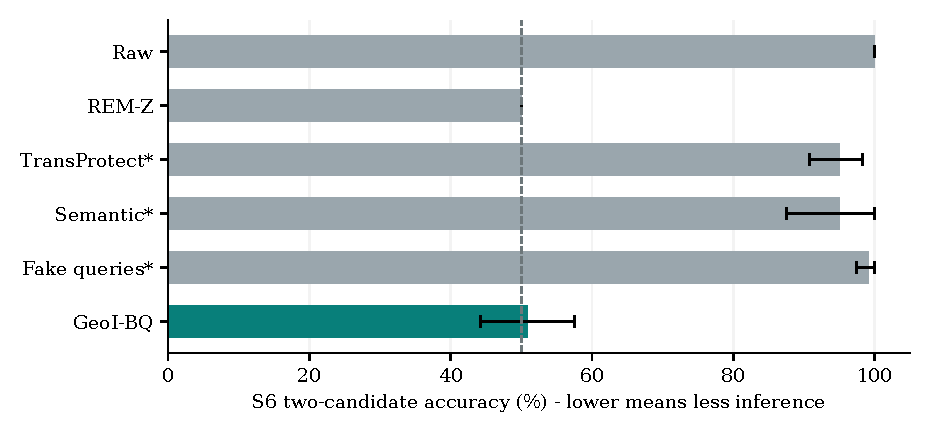
\includegraphics[width=\linewidth]{figures/future_choice.pdf}
\caption{S6 sau rẽ: accuracy chọn đích với CI95\%. Đường đứt là mốc uniform 50\% của hai lựa chọn.}
\label{fig:future}
\end{figure}

Hai task S5/S6 dùng cùng private route-choice bit trong workload; không được đếm như hai nguồn
bằng chứng hoàn toàn độc lập. Các pha, Brier và log loss đầy đủ ở Phụ lục~\ref{app:extended}.
Một tác vụ S6 dùng sáu chuyến lịch sử đã bảo vệ chưa chạy vì frozen outputs chỉ có ngày 7/8;
không dùng native lịch sử chưa bảo vệ để lấp vào như cùng contract.

\subsection{S7: kiểm tra payload có điều kiện}
Giữ cùng GPS/Q, clock và provider; thay bốn purposes nhân sáu categories tại local. Kiểm tra
\path{SessionCoverClient} thực qua provider probe trả reply rỗng cố định; actual frozen reply-mask
signatures được xác thực riêng. Đây là audit interface/payload, không chạy lại utility POI hoặc
huấn luyện một natural-intent attacker.
\Needspace{210pt}
\par\begingroup\small\setstretch{1.04}\setlength{\parskip}{0pt}
\begin{longtable}{@{}P{3.2cm}P{2.919cm}P{2.919cm}P{2.919cm}P{2.919cm}@{}}
\caption{S7: độ phân biệt payload có điều kiện trong common wrapper}\label{tab:s7}\\
\toprule
\textbf{Phương pháp} & \textbf{Wire bằng nhau} & \textbf{Purpose\%} & \textbf{Category\%} & \textbf{Joint\%} \\
\midrule\endfirsthead
\multicolumn{5}{l}{\small\textit{Bảng \thetable\ (tiếp)}}\\\toprule
\textbf{Phương pháp} & \textbf{Wire bằng nhau} & \textbf{Purpose\%} & \textbf{Category\%} & \textbf{Joint\%} \\
\midrule\endhead
\midrule\multicolumn{5}{r}{\small\textit{Còn tiếp ở trang sau}}\\\endfoot
\bottomrule\endlastfoot
Raw GPS & 100{,}00 & 25{,}00 & 16{,}67 & 4{,}17 \\
REM-Z K1 & 100{,}00 & 25{,}00 & 16{,}67 & 4{,}17 \\
TransProtect* & 100{,}00 & 25{,}00 & 16{,}67 & 4{,}17 \\
Semantic correlation* & 100{,}00 & 25{,}00 & 16{,}67 & 4{,}17 \\
Fake-query insertion* & 100{,}00 & 25{,}00 & 16{,}67 & 4{,}17 \\
\textbf{GeoI-BQ v1} & 100{,}00 & 25{,}00 & 16{,}67 & 4{,}17 \\
\end{longtable}\endgroup\par


Cả 1.056 streams đều có wire bằng nhau, tương ứng 25.344 counterfactuals. Với prior cân bằng,
conditional Bayes vulnerability là purpose 25\%, category 16,67\%, joint 4,17\%.
Control đưa purpose/category trực tiếp vào request khôi phục 100\% nhãn joint. Tất cả sáu arm dùng
chung cover wrapper, nên đây là tính chất của interface chung, không là ưu thế riêng của GeoI-BQ
trước implementation gốc của paper. Ý định gắn với tuyến, account hoặc lúc mở phiên vẫn có thể
được suy luận và chưa được đo ở đây.

\subsection{S8: hai kênh có prefix tương quan}
Dùng hai phiên native ngày 7/8 khác nhau cùng family, căn theo clock tương đối và cắt tại public
tick trước fork. GPS hai phiên giống nhau trên prefix đó. Attacker được cấp association giữa hai
kênh. Đây là \textbf{tương quan tổng hợp hoàn hảo sau căn clock}, không phải dữ liệu hai xe đồng
hành chạy đồng thời, cũng không là kết quả companion detection.

Bốn views là target-only, thêm protected partner, thêm Raw partner và thêm protected partner từ
family khác trong block. Target là GPS tại cutoff; mọi feature chỉ dùng causal prefix. Bảng dưới
dùng bank fusion V2, mỗi ô Hit100\% / MAE m; các loss được chọn attacker riêng.
\Needspace{210pt}
\par\begingroup\small\setstretch{1.04}\setlength{\parskip}{0pt}
\begin{longtable}{@{}P{3.2cm}P{2.919cm}P{2.919cm}P{2.919cm}P{2.919cm}@{}}
\caption{S8 với attacker fusion: Hit100 (\%) / MAE (m)}\label{tab:s8}\\
\toprule
\textbf{Phương pháp} & \textbf{Target} & \textbf{+ protected} & \textbf{+ raw} & \textbf{+ unrelated} \\
\midrule\endfirsthead
\multicolumn{5}{l}{\small\textit{Bảng \thetable\ (tiếp)}}\\\toprule
\textbf{Phương pháp} & \textbf{Target} & \textbf{+ protected} & \textbf{+ raw} & \textbf{+ unrelated} \\
\midrule\endhead
\midrule\multicolumn{5}{r}{\small\textit{Còn tiếp ở trang sau}}\\\endfoot
\bottomrule\endlastfoot
Raw GPS & 100{,}00 / 0{,}0 & 100{,}00 / 0{,}0 & 100{,}00 / 0{,}0 & 100{,}00 / 0{,}0 \\
REM-Z K1 & 10{,}83 / 359{,}7 & 6{,}67 / 300{,}8 & 100{,}00 / 0{,}0 & 10{,}83 / 359{,}7 \\
TransProtect* & 60{,}83 / 102{,}8 & 64{,}17 / 96{,}8 & 98{,}33 / 0{,}0 & 60{,}83 / 102{,}8 \\
Semantic correlation* & 45{,}00 / 101{,}4 & 75{,}00 / 46{,}2 & 100{,}00 / 0{,}0 & 45{,}00 / 101{,}4 \\
Fake-query insertion* & 16{,}67 / 1857{,}4 & 68{,}33 / 1857{,}4 & 100{,}00 / 0{,}0 & 16{,}67 / 1857{,}4 \\
\textbf{GeoI-BQ v1} & 0{,}00 / 2246{,}7 & 0{,}00 / 2226{,}8 & 100{,}00 / 0{,}0 & 0{,}00 / 2246{,}7 \\
\end{longtable}\endgroup\par


GeoI-BQ không có hit trong mẫu target/+protected, với MAE lần lượt 2.246,7 và 2.226,8 m.
Điều đó không chứng minh risk bằng không; bootstrap [0;0] khi mẫu toàn không-hit chỉ phản ánh
giới hạn của resampling mẫu đó. Khi Raw partner được cấp, estimator đọc partner trực tiếp có
Hit100 100\% ở mọi arm vì GPS prefix trùng nhau. Selected estimator TransProtect* đạt 98,33\%
Hit100 ở TEST, còn MAE 0 thuộc một estimator khác; các arm còn lại selected Hit100 là 100\%.
Không gộp hai selected losses thành một attacker duy nhất.

Kết quả cho thấy raw side information rất mạnh có thể làm mất vị trí mục tiêu dù target stream
đã bảo vệ. Một guard single-session không tự chứng nhận nhiều kênh/người cùng lúc. View unrelated
giúp kiểm tra rằng phép ghép ngẫu nhiên không tạo cùng tín hiệu; nó chưa mô hình hóa mọi dạng
tương quan mềm hoặc auxiliary data thực tế.

\subsection{Tăng cường attacker S8: giữ cả V1 và V2}
V1 có ExtraTrees64, kNN, prior, centroid/velocity và luôn giữ target-only estimators trong joint
bank. Sau khi xem V1, audit nhận ra còn thiếu phép fusion đơn giản. V2 giữ V1 rồi thêm trung bình
centroid/median/velocity hai kênh với trọng số $1/4,1/2,3/4$, midpoint của cặp Q gần nhất và trung
bình hai/ba cặp gần nhất. Nếu hai tập cùng chứa GPS thật, đối chiếu hai tập có thể lộ thành viên đó.
Không dùng GPS target, nhãn real/fake hoặc evaluator IDs để tìm cặp.
\Needspace{210pt}
\par\begingroup\small\setstretch{1.04}\setlength{\parskip}{0pt}
\begin{longtable}{@{}P{3.1cm}P{2.944cm}P{2.944cm}P{2.944cm}P{2.944cm}@{}}
\caption{S8 protected-partner: V1 và vòng attacker fusion V2}\label{tab:fusion}\\
\toprule
\textbf{Phương pháp} & \textbf{V1 Hit\%} & \textbf{V2 Hit\%} & \textbf{V1 MAE m} & \textbf{V2 MAE m} \\
\midrule\endfirsthead
\multicolumn{5}{l}{\small\textit{Bảng \thetable\ (tiếp)}}\\\toprule
\textbf{Phương pháp} & \textbf{V1 Hit\%} & \textbf{V2 Hit\%} & \textbf{V1 MAE m} & \textbf{V2 MAE m} \\
\midrule\endhead
\midrule\multicolumn{5}{r}{\small\textit{Còn tiếp ở trang sau}}\\\endfoot
\bottomrule\endlastfoot
Raw GPS & 100{,}00 & 100{,}00 & 0{,}0 & 0{,}0 \\
REM-Z K1 & 10{,}83 & 6{,}67 & 359{,}7 & 300{,}8 \\
TransProtect* & 60{,}83 & 64{,}17 & 102{,}8 & 96{,}8 \\
Semantic correlation* & 45{,}00 & 75{,}00 & 101{,}4 & 46{,}2 \\
Fake-query insertion* & 16{,}67 & 68{,}33 & 1857{,}4 & 1857{,}4 \\
\textbf{GeoI-BQ v1} & 0{,}00 & 0{,}00 & 2226{,}8 & 2226{,}8 \\
\end{longtable}\endgroup\par


Semantic* tăng Hit100 từ 45 lên 75\%; Fake-query* từ 16,67 lên 68,33\%. Điều này minh họa vì sao
một attacker bank thiếu thao tác cơ bản có thể làm defense trông mạnh hơn. REM-Z có MAE giảm nhưng
selected Hit100 cũng giảm ở TEST; selection đúng protocol không bảo đảm mọi loss TEST đều cải thiện.
V2 được chốt sau readout V1 và chọn trên SELECTION: đây là post-V1 diagnostic trên cùng dữ liệu
đã xem, không phải confirmation độc lập.

\begin{figure}[htbp]\centering
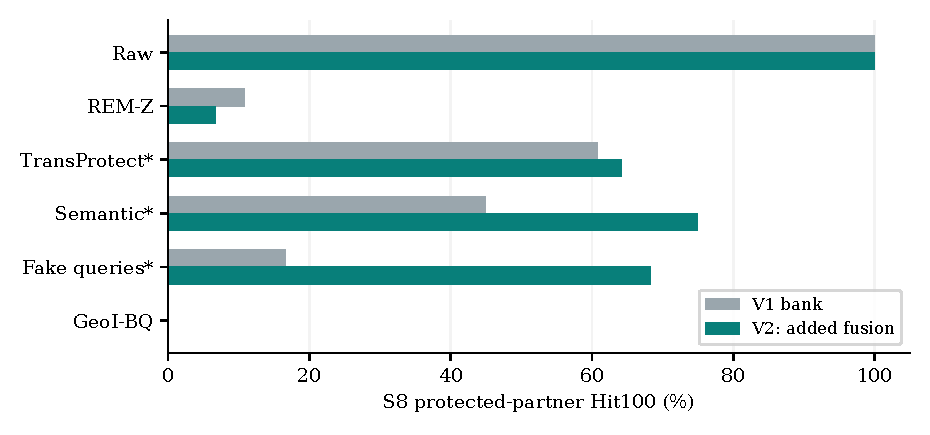
\includegraphics[width=\linewidth]{figures/joint_attack_fusion.pdf}
\caption{S8 protected-partner: readout V1 và V2. Fusion bổ sung làm rõ rủi ro giao hai tập chứa GPS thật.}
\label{fig:fusion}
\end{figure}

Verifier V2 ban đầu đặt gate selected Raw-partner Hit100 phải bằng 100\% ở mọi arm. Một fusion
estimator có tie tốt trên SELECTION chỉ đạt 98,33\% ở TransProtect* TEST; available
\path{partner_centroid} vẫn đạt 100\%. Giữ failure gốc và dùng checker độc lập kiểm tra cả available
control lẫn selected score. Không sửa predictions hoặc defense để thỏa gate sai. Chi tiết replay
ở Phụ lục~\ref{app:repro}.

\subsection{Tổng hợp mức hoàn thành theo scenario}
\begin{longtable}{@{}P{1cm}P{5.0cm}P{9.4cm}@{}}
\caption{Mức bằng chứng hiện có; không đồng nhất coverage với bảo vệ tuyệt đối.}\label{tab:scenario-status}\\
\toprule Case & Bằng chứng hiện có & Điều chưa được kết luận\\\midrule\endfirsthead
\toprule Case & Bằng chứng hiện có & Điều chưa được kết luận\\\midrule\endhead
\bottomrule\endfoot
S1 & Isolated-event Hit100/MAE & Không là chứng nhận mọi snapshot attacker.\\
S2 & Late-window coordinate proxy & Chưa suy luận semantic stop/home/work.\\
S3 & Whole-window reconstruction & Không là xác nhận ngoài cohort/thành phố.\\
S4 & Route-family association và odds có điều kiện & Nhãn người/xe vật lý, account anonymity còn N/A.\\
S5 & Causal two-edge diagnostic & Raw chance: chưa tách đóng góp defense.\\
S6 & Two-destination post-turn, Raw có tín hiệu & Unrestricted destination/routine history còn ngoài trial.\\
S7 & Conditional payload noninterference & Natural intent hoặc route-correlated purpose chưa đo.\\
S8 & Aligned correlated channels, bank fusion & Native co-travel, association detection và joint theorem riêng.\\
S9 & First GPS từ toàn transcript & Không dựa vào giấu public start clock.\\
S10 & Last GPS từ toàn transcript & Không dựa vào giấu end clock hoặc bỏ packet cuối bằng delay.\\
\end{longtable}
